\par En esta secci\'on realizaremos un an\'alisis cualitativo de los m\'etodos desarrollados.
Con este fin, observaremos el resultado de aplicar los distintos m\'etodos a ciertas entradas; 
buscaremos \textit{artifacts} (errores visibles en el video causados por la interpolaci\'on), compararemos los diferentes procedimientos entre s\'i, y los efectos de distintos par\'ametros en cada uno.

\subsubsection{Artifacts}
\par Si bien encontrar una interpolaci\'on ideal puede no ser posible, se pueden generar frames intermedios que no sean completamentamente fidedignos a los id\'oneos, pero que son de todas formas veros\'imiles.
Un objetivo quiz\'as m\'as plausible que una interpolaci\'on perfecta o ideal, es una de la cual el observador no puede discernir de los frames originales (al menos en una observaci\'on ``normal''). 
Los \textit{artifacts} son errores en la interpolaci\'on que tienen un efecto visible en el video, y que detraen de este objetivo. 
Los estudiaremos con especial atenci\'on ya que tienen un significativo efecto negativo en la percibida calidad del video resultante.

\subsubsubsection{Vecino m\'as cercano}
\par La mayor\'ia de los m\'etodos de interpolaci\'on intentan ``adivinar'' los frames intermedios en base a los de referencia, lo que conlleva posibles errores.
Vecino m\'as cercano, por otro lado, genera a los intermedios copiando a los de referencia, por lo que no se pueden producir artifacts.

\subsubsubsection{Lineal y Splines}
\par Ambos m\'etodos funcionan de forma similar: viendo c\'omo var\'ian los valores de los mismo p\'ixeles (es decir, de los p\'ixeles que est\'an en la misma posici\'on de cada frame) entre los frames de referencia, e interpolando los valores de los intermedios.
Lo que var\'ia es la familia de funciones mediante la cual aproximan, y cu\'antos frames de referencia utilizan.
Debido a esto, ambos m\'etodos generan ``trazas'' al interpolar movimiento.
A continuaci\'on ahondaremos en esto, y daremos ejemplos.

\subsubsubsection{Lineal}
\par Si el video representa el movimiento (algo casi ubicuo en este tipo de aplicaciones) de alg\'un cuerpo a lo largo de los frames, lo que este m\'etodo hace es esencialmente un ``fade-in'' y ``fade-out'' del objeto del primer frame de referencia al segundo.
Para clarificar lo anterior: se observa que el objeto en el primer frame se va transformando en el fondo (en la posici\'on de dicho objeto) del segundo, mientras que el fondo (en la nueva posici\'on del objeto) del primero se va transformando en el objeto del segundo.
\par En la realidad (a escala no-cu\'antica), el movimiento es continuo, por lo que idealmente la interpolaci\'on deber\'ia generar frames intermedios donde el cuerpo en movimiento se encuentra en los puntos intermedios de dicho movimiento.
El m\'etodo lineal genera movimiento discontinuo, donde el cuerpo se funde de una posici\'on en un frame de referencia a la del pr\'oximo frame.
Un claro ejemplo de estas trazas o ``fade-in''-``fade-out'' se puede observar en la imagen \ref{TenisTrazaLineal}, que es un frame interpolado linealmente.

\FloatBarrier
\begin{figure}[h]
\caption{Traza en interpolacion lineal}
\label{TenisTrazaLineal}
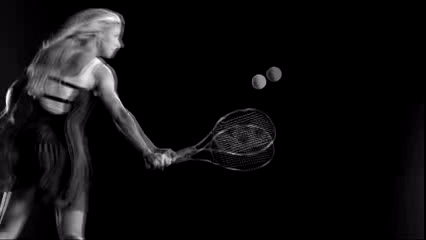
\includegraphics[width=0.9\columnwidth]{imagenes/cualitativos/TTL.png}
\end{figure}
\FloatBarrier

\par Si bien estas trazas t\'ecnicamente son artifacts, ya que no representan la realidad del video, cabe destacar que a los seres humanos \'estas no nos parecen muy fuera de lugar o inveros\'imiles; en dibujo, efectos especiales y dem\'as, una forma de representar movimiento es justamente mediante tales trazas; incluso nuestro propio sentido de visi\'on en ciertas circunstancias captura el movimiento de tal forma (como cualquiera habr\'a hecho en alg\'un momento, si uno mueve la mano r\'apidamente de un lado al otro con el brazo fijo se observan trazas en vez de un movimiento continuo - otro ejemplo es el cl\'asico truco del l\'apiz que parece hecho de goma). 
\par Debido a esto, las trazas pueden tener un impacto incluso positivo en el video en lo que concierne a interpolaci\'on del movimiento, en especial con framerate alto y pocos frames intermedios.

\subsubsubsection{Splines}
\par En el m\'etodo de Splines se observan trazas similares a las de la interpolaci\'on lineal; la diferencia yace en c\'omo se ve el ``fade-in''-``fade-out''.
Un ejemplo de tales trazas, para el mismo video que el de la imagen \ref{TenisTrazaLineal}, se encuentra en la figura \ref{TenisTrazaSplines}.

\FloatBarrier
\begin{figure}[h]
\caption{Traza en Splines}
\label{TenisTrazaSplines}
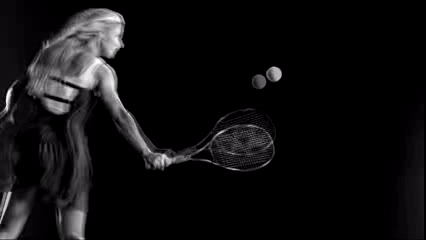
\includegraphics[width=0.9\columnwidth]{imagenes/cualitativos/TTS.png}
\end{figure}
\FloatBarrier

\par Cabe destacar que las trazas en Splines se ven con mayor claridad al incrementar el tama\~no de bloque.
Se observa que esto detrae del efecto positivo mencionado previamente.

\subsubsection{Cambio de Escena}
\par Los componentes (en el sentido, de objetos, cuerpos, paisajes y dem\'as) de un video pueden pasar de un frame al otro esencialmente de tres maneras: 
se pueden quedar quietos (en cuyo caso los tres m\'etodos empleados las mantendr\'an iguales como deben, y por ende sin artifacts),
se pueden mover de alg\'un lugar del video al otro (los efectos de los m\'etodos de interpolaci\'on en el movimiento fueron detallados en la secci\'on previa),
o pueden aparecer/desaparecer (o saltar de un lugar a otro de una forma discontinua).
\par Cuando desaparece toda la escena y aparece una enteramente nueva, se dice que hubo un cambio de escena.
\'Este es el caso que analizaremos, ya que en las im\'agenes resultantes se ve con mayor claridad los efectos de los distintos m\'etodos de interpolaci\'on, pero todo lo que detallaremos en esta secci\'on se aplica perfectamente en el caso de que s\'olo algunos componentes aparezcan o desaparezcan.
\par El caso de cambio de escena es distinto que el de movimiento (real, el ficticio que no necesariamente es continuo lo contemplamos como aparici\'on/desaparici\'on por lo que se detallar\'a a continuaci\'on), ya que no necesariamente sabemos que es una transici\'on continua. 
Es perfectamente posible que la transici\'on de escenas sea un ``fade-out'' de una y un ``fade-in'' de otra, o que sea un corte limpio en el cual todo frame pertenece exclusivamente a una u otra (de hecho, ambas transiciones son usadas ampliamente en la cinematograf\'ia), o incluso mediante alguna otra t\'ecnica (como ejemplo, considerar las distintas formas de pasar de una diapositiva a otra en PowerPoint).
Adicionalmente, en ciertos casos es directamente imposible determinar cu\'al m\'etodo de transici\'on se utiliz\'o realmente (por ejemplo si el input es un subconjunto de frames de un cierto video original, y s\'olo se tienen frames anteriores y posteriores a la transici\'on).
\par Debido a esto, no consideraremos la forma en que los m\'etodos terminan efectuando el cambio de escena como errores o artifacts.
De todas modos, observaremos tales formas como parte de nuestro an\'alisis cualitativo.

\subsubsubsection{Vecino m\'as cercano}
\par Los frames intermedios a los de dos escenas distintas (es decir, los que representan tal cambio de escena) en este m\'etodo ser\'an copias del frame m\'as cercano, por lo que resultar\'an en una transici\'on ``limpia'', repentina, que pasa de una escena a la otra sin frames que pertenecen a ambas.

\subsubsubsection{Lineal y Splines}
\par El m\'etodo lineal resultar\'a en un ``fade-in''-``fade-out'' entre las escenas, con todos los frames intermedios pertenecientes a ambas.
Un ejemplo de esta transici\'on se puede ver en la imagen \ref{BebesLinealTransicion}, que corresponde a un frame intermedio a dos escenas distintas (en la escena saliente se ve al beb\'e con mayor zoom, en la entrante con menor).

\FloatBarrier
\begin{figure}[h]
\caption{Transicion Lineal}
\label{BebesLinealTransicion}
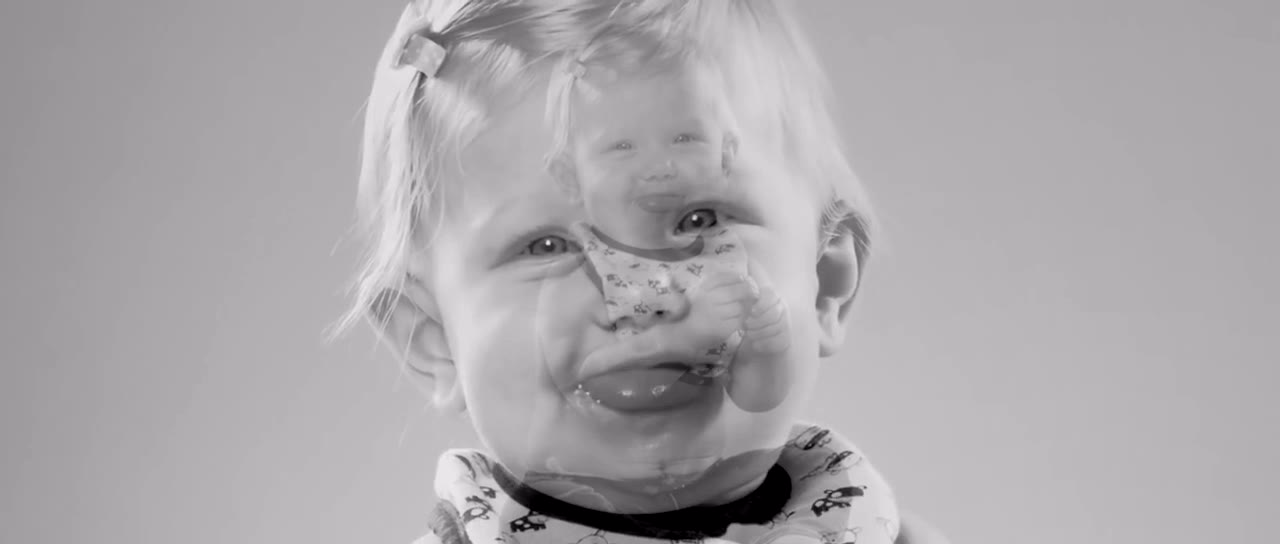
\includegraphics[width=0.9\columnwidth]{imagenes/cualitativos/BLT.png}
\end{figure}
\FloatBarrier

\par El uso de Splines resulta en el mismo tipo de transici\'on que la interpolaci\'on lineal (ejemplo: figura \ref{BebesSplinesTransicion}).
Nuevamente, la diferencia entre ambos yace en la intensidad de cada escena en el ``fade-in''-``fade-out''.

\FloatBarrier
\begin{figure}[h]
\caption{Transicion en Splines}
\label{BebesSplinesTransicion}
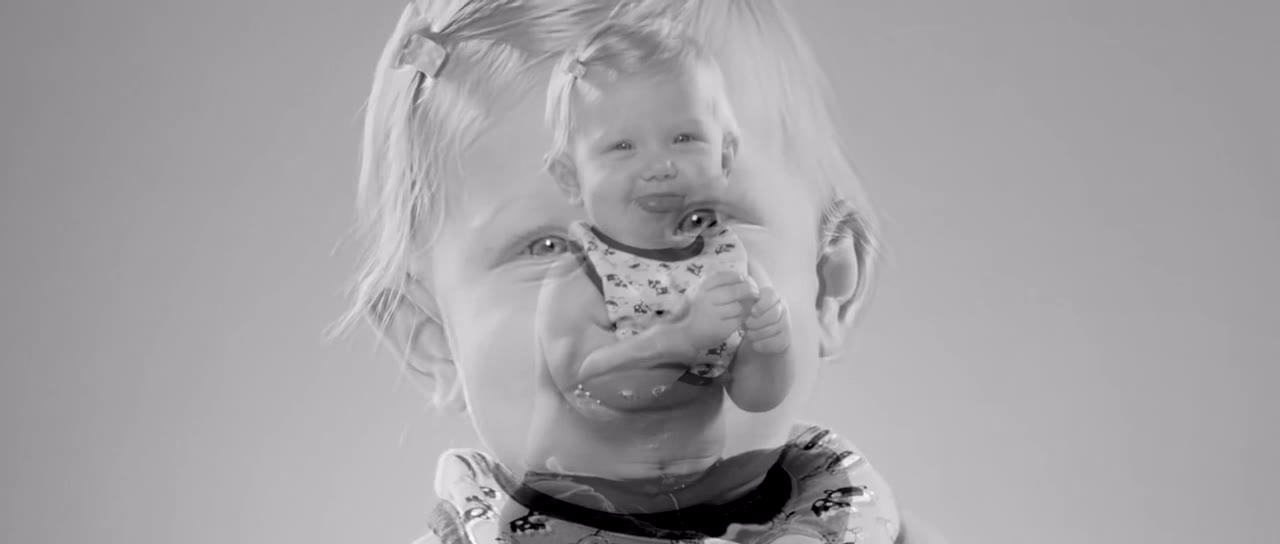
\includegraphics[width=0.9\columnwidth]{imagenes/cualitativos/BST.png}
\end{figure}
\FloatBarrier

\par Sin embargo, Splines utiliza varios frames de referencia, por lo que en algunos casos otra escena puede alterar frames que no son de transici\'on de una a otra.
Esto resulta en artifacts, como el que se puede observar en la figura \ref{BebesSplinesArtifact}.
Cabe destacar que la frecuencia y el efecto de este artifact incrementar al aumentar el tama\~no de bloque.

\FloatBarrier
\begin{figure}[h]
\caption{Artifact de transicion en Splines}
\label{BebesSplinesArtifact}

\includegraphics[width=0.9\columnwidth]{imagenes/cualitativos/BSA.png}
\end{figure}
\FloatBarrier

\subsubsection{Comparaci\'on de la calidad de los m\'etodos}
\par En lo que concierne a Splines y Lineal contra Vecino m\'as cercano, observamos que el efecto de trazas presente en los primeros genera un efecto m\'as din\'amico y fluido en los videos, en contraposici\'on al efecto m\'as est\'atico de este \'ultimo.
Si bien la decisi\'on de cu\'al es mejor es subjetiva, personalmente nos pareci\'o que en videos de movimiento, Splines y Lineal eran mejores.
En videos que consisten mayoritariamente de cambios de escena (un slideshow de fotos, por ejemplo), depende de la opinion personal de cada uno con respecto al m\'etodo de transici\'on preferido.
\par En lo que concierne a Splines y Lineal, observamos que la traza es m\'as visible (se nota m\'as desde el punto de vista conciente), y nos pareci\'o que era preferible la traza m\'as sutil de interpolaci\'on lineal.
Esto, junto a los artifacts de transici\'on en Splines, nos llevan a recomendar la interpolaci\'on lineal por sobre este m\'etodo.
